\documentclass[twoside]{book}

% Packages required by doxygen
\usepackage{fixltx2e}
\usepackage{calc}
\usepackage{doxygen}
\usepackage[export]{adjustbox} % also loads graphicx
\usepackage{graphicx}
\usepackage[utf8]{inputenc}
\usepackage{makeidx}
\usepackage{multicol}
\usepackage{multirow}
\PassOptionsToPackage{warn}{textcomp}
\usepackage{textcomp}
\usepackage[nointegrals]{wasysym}
\usepackage[table]{xcolor}

% Font selection
\usepackage[T1]{fontenc}
\usepackage[scaled=.90]{helvet}
\usepackage{courier}
\usepackage{amssymb}
\usepackage{sectsty}
\renewcommand{\familydefault}{\sfdefault}
\allsectionsfont{%
  \fontseries{bc}\selectfont%
  \color{darkgray}%
}
\renewcommand{\DoxyLabelFont}{%
  \fontseries{bc}\selectfont%
  \color{darkgray}%
}
\newcommand{\+}{\discretionary{\mbox{\scriptsize$\hookleftarrow$}}{}{}}

% Page & text layout
\usepackage{geometry}
\geometry{%
  a4paper,%
  top=2.5cm,%
  bottom=2.5cm,%
  left=2.5cm,%
  right=2.5cm%
}
\tolerance=750
\hfuzz=15pt
\hbadness=750
\setlength{\emergencystretch}{15pt}
\setlength{\parindent}{0cm}
\setlength{\parskip}{3ex plus 2ex minus 2ex}
\makeatletter
\renewcommand{\paragraph}{%
  \@startsection{paragraph}{4}{0ex}{-1.0ex}{1.0ex}{%
    \normalfont\normalsize\bfseries\SS@parafont%
  }%
}
\renewcommand{\subparagraph}{%
  \@startsection{subparagraph}{5}{0ex}{-1.0ex}{1.0ex}{%
    \normalfont\normalsize\bfseries\SS@subparafont%
  }%
}
\makeatother

% Headers & footers
\usepackage{fancyhdr}
\pagestyle{fancyplain}
\fancyhead[LE]{\fancyplain{}{\bfseries\thepage}}
\fancyhead[CE]{\fancyplain{}{}}
\fancyhead[RE]{\fancyplain{}{\bfseries\leftmark}}
\fancyhead[LO]{\fancyplain{}{\bfseries\rightmark}}
\fancyhead[CO]{\fancyplain{}{}}
\fancyhead[RO]{\fancyplain{}{\bfseries\thepage}}
\fancyfoot[LE]{\fancyplain{}{}}
\fancyfoot[CE]{\fancyplain{}{}}
\fancyfoot[RE]{\fancyplain{}{\bfseries\scriptsize Generated by Doxygen }}
\fancyfoot[LO]{\fancyplain{}{\bfseries\scriptsize Generated by Doxygen }}
\fancyfoot[CO]{\fancyplain{}{}}
\fancyfoot[RO]{\fancyplain{}{}}
\renewcommand{\footrulewidth}{0.4pt}
\renewcommand{\chaptermark}[1]{%
  \markboth{#1}{}%
}
\renewcommand{\sectionmark}[1]{%
  \markright{\thesection\ #1}%
}

% Indices & bibliography
\usepackage{natbib}
\usepackage[titles]{tocloft}
\setcounter{tocdepth}{3}
\setcounter{secnumdepth}{5}
\makeindex

% Hyperlinks (required, but should be loaded last)
\usepackage{ifpdf}
\ifpdf
  \usepackage[pdftex,pagebackref=true]{hyperref}
\else
  \usepackage[ps2pdf,pagebackref=true]{hyperref}
\fi
\hypersetup{%
  colorlinks=true,%
  linkcolor=blue,%
  citecolor=blue,%
  unicode%
}

% Custom commands
\newcommand{\clearemptydoublepage}{%
  \newpage{\pagestyle{empty}\cleardoublepage}%
}

\usepackage{caption}
\captionsetup{labelsep=space,justification=centering,font={bf},singlelinecheck=off,skip=4pt,position=top}

%===== C O N T E N T S =====

\begin{document}

% Titlepage & ToC
\hypersetup{pageanchor=false,
             bookmarksnumbered=true,
             pdfencoding=unicode
            }
\pagenumbering{alph}
\begin{titlepage}
\vspace*{7cm}
\begin{center}%
{\Large I\+OT Devices Client -\/ Server Communication System }\\
\vspace*{1cm}
{\large Generated by Doxygen 1.8.13}\\
\end{center}
\end{titlepage}
\clearemptydoublepage
\pagenumbering{roman}
\tableofcontents
\clearemptydoublepage
\pagenumbering{arabic}
\hypersetup{pageanchor=true}

%--- Begin generated contents ---
\chapter{Hierarchical Index}
\section{Class Hierarchy}
This inheritance list is sorted roughly, but not completely, alphabetically\+:\begin{DoxyCompactList}
\item \contentsline{section}{iotserver.\+Database}{\pageref{classiotserver_1_1Database}}{}
\item \contentsline{section}{iotclient.\+Iotclient}{\pageref{classiotclient_1_1Iotclient}}{}
\item \contentsline{section}{iotserver.\+Iotserver}{\pageref{classiotserver_1_1Iotserver}}{}
\item \contentsline{section}{iotclient.\+Message}{\pageref{classiotclient_1_1Message}}{}
\item Thread\begin{DoxyCompactList}
\item \contentsline{section}{iotserver.\+Client\+Handler}{\pageref{classiotserver_1_1ClientHandler}}{}
\end{DoxyCompactList}
\end{DoxyCompactList}

\chapter{Class Index}
\section{Class List}
Here are the classes, structs, unions and interfaces with brief descriptions\+:\begin{DoxyCompactList}
\item\contentsline{section}{\hyperlink{classiotserver_1_1ClientHandler}{iotserver.\+Client\+Handler} }{\pageref{classiotserver_1_1ClientHandler}}{}
\item\contentsline{section}{\hyperlink{classiotserver_1_1Database}{iotserver.\+Database} }{\pageref{classiotserver_1_1Database}}{}
\item\contentsline{section}{\hyperlink{classiotclient_1_1Iotclient}{iotclient.\+Iotclient} }{\pageref{classiotclient_1_1Iotclient}}{}
\item\contentsline{section}{\hyperlink{classiotserver_1_1Iotserver}{iotserver.\+Iotserver} }{\pageref{classiotserver_1_1Iotserver}}{}
\item\contentsline{section}{\hyperlink{classiotclient_1_1Message}{iotclient.\+Message} }{\pageref{classiotclient_1_1Message}}{}
\end{DoxyCompactList}

\chapter{Class Documentation}
\hypertarget{classiotserver_1_1ClientHandler}{}\section{iotserver.\+Client\+Handler Class Reference}
\label{classiotserver_1_1ClientHandler}\index{iotserver.\+Client\+Handler@{iotserver.\+Client\+Handler}}


Inheritance diagram for iotserver.\+Client\+Handler\+:\nopagebreak
\begin{figure}[H]
\begin{center}
\leavevmode
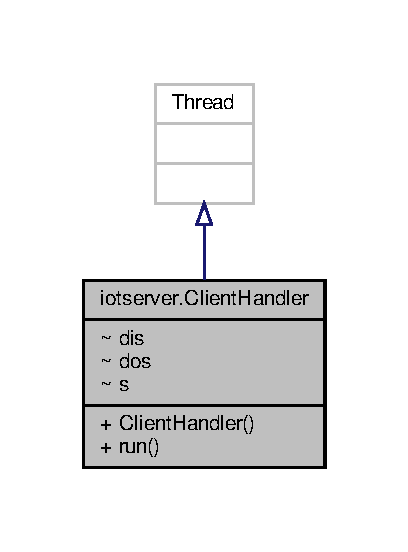
\includegraphics[width=196pt]{classiotserver_1_1ClientHandler__inherit__graph}
\end{center}
\end{figure}


Collaboration diagram for iotserver.\+Client\+Handler\+:\nopagebreak
\begin{figure}[H]
\begin{center}
\leavevmode
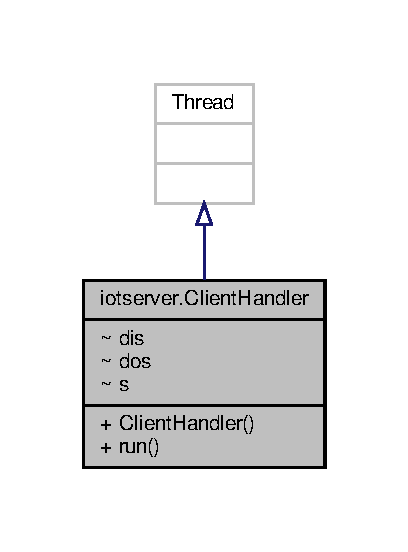
\includegraphics[width=196pt]{classiotserver_1_1ClientHandler__coll__graph}
\end{center}
\end{figure}
\subsection*{Public Member Functions}
\begin{DoxyCompactItemize}
\item 
\mbox{\Hypertarget{classiotserver_1_1ClientHandler_a398c6a2929211d5a5195097e4be514f4}\label{classiotserver_1_1ClientHandler_a398c6a2929211d5a5195097e4be514f4}} 
{\bfseries Client\+Handler} (Socket s, Data\+Input\+Stream dis, Data\+Output\+Stream dos)
\item 
\mbox{\Hypertarget{classiotserver_1_1ClientHandler_a789667c4064f8281f810a02bcde2ba1f}\label{classiotserver_1_1ClientHandler_a789667c4064f8281f810a02bcde2ba1f}} 
void {\bfseries run} ()
\end{DoxyCompactItemize}


The documentation for this class was generated from the following file\+:\begin{DoxyCompactItemize}
\item 
/home/ivica/\+Coding/\+Java/\+C\+S\+\_\+\+I\+O\+T/iotserver/src/iotserver/Client\+Handler.\+java\end{DoxyCompactItemize}

\hypertarget{classiotserver_1_1Database}{}\section{iotserver.\+Database Class Reference}
\label{classiotserver_1_1Database}\index{iotserver.\+Database@{iotserver.\+Database}}


Collaboration diagram for iotserver.\+Database\+:\nopagebreak
\begin{figure}[H]
\begin{center}
\leavevmode
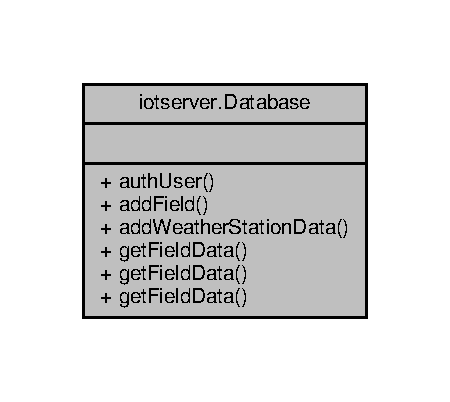
\includegraphics[width=216pt]{classiotserver_1_1Database__coll__graph}
\end{center}
\end{figure}
\subsection*{Public Member Functions}
\begin{DoxyCompactItemize}
\item 
boolean \hyperlink{classiotserver_1_1Database_a2a4ab1640565d077045f9867c59a2573}{auth\+User} (String username, String password)
\item 
J\+S\+O\+N\+Object \hyperlink{classiotserver_1_1Database_ac0c9d5c5ea706160d836578c8019d1a7}{add\+Field} (String field\+Name, double latitude, double longitude)
\item 
boolean \hyperlink{classiotserver_1_1Database_ae7dfbdcecabac722a8f3ef63a73559b5}{add\+Weather\+Station\+Data} (long weather\+Station\+Id, double temperature, double barometric\+Pressure, double wind\+Speed, double relative\+Humidity, long air\+Quality\+Index)
\item 
J\+S\+O\+N\+Object \hyperlink{classiotserver_1_1Database_a2c12fba48ac94748e7ce8fb412b19c1e}{get\+Field\+Data} (String field\+Name)
\item 
J\+S\+O\+N\+Object \hyperlink{classiotserver_1_1Database_ac968e2f70df507390dcd535660801c5e}{get\+Field\+Data} (Connection db, String field\+Name)
\item 
J\+S\+O\+N\+Array \hyperlink{classiotserver_1_1Database_ab92010b913a502847e7a062d2aa9ad72}{get\+Field\+Data} ()
\end{DoxyCompactItemize}


\subsection{Member Function Documentation}
\mbox{\Hypertarget{classiotserver_1_1Database_ac0c9d5c5ea706160d836578c8019d1a7}\label{classiotserver_1_1Database_ac0c9d5c5ea706160d836578c8019d1a7}} 
\index{iotserver\+::\+Database@{iotserver\+::\+Database}!add\+Field@{add\+Field}}
\index{add\+Field@{add\+Field}!iotserver\+::\+Database@{iotserver\+::\+Database}}
\subsubsection{\texorpdfstring{add\+Field()}{addField()}}
{\footnotesize\ttfamily J\+S\+O\+N\+Object iotserver.\+Database.\+add\+Field (\begin{DoxyParamCaption}\item[{String}]{field\+Name,  }\item[{double}]{latitude,  }\item[{double}]{longitude }\end{DoxyParamCaption})\hspace{0.3cm}{\ttfamily [inline]}}

Function that accesses database in order to add field to the system.


\begin{DoxyParams}{Parameters}
{\em field\+Name} & Name of the field, as string \\
\hline
{\em latitude} & Geographical latitude, as double number \\
\hline
{\em longitude} & Geographical longitude, as double number \\
\hline
\end{DoxyParams}
\begin{DoxyReturn}{Returns}
J\+S\+O\+N\+Object containing data about entered field 
\end{DoxyReturn}
\mbox{\Hypertarget{classiotserver_1_1Database_ae7dfbdcecabac722a8f3ef63a73559b5}\label{classiotserver_1_1Database_ae7dfbdcecabac722a8f3ef63a73559b5}} 
\index{iotserver\+::\+Database@{iotserver\+::\+Database}!add\+Weather\+Station\+Data@{add\+Weather\+Station\+Data}}
\index{add\+Weather\+Station\+Data@{add\+Weather\+Station\+Data}!iotserver\+::\+Database@{iotserver\+::\+Database}}
\subsubsection{\texorpdfstring{add\+Weather\+Station\+Data()}{addWeatherStationData()}}
{\footnotesize\ttfamily boolean iotserver.\+Database.\+add\+Weather\+Station\+Data (\begin{DoxyParamCaption}\item[{long}]{weather\+Station\+Id,  }\item[{double}]{temperature,  }\item[{double}]{barometric\+Pressure,  }\item[{double}]{wind\+Speed,  }\item[{double}]{relative\+Humidity,  }\item[{long}]{air\+Quality\+Index }\end{DoxyParamCaption})\hspace{0.3cm}{\ttfamily [inline]}}

Function that enters weather station data to a weather\+Station\+Data table.

Data entered to a table depends on the arguments provided to this method. Function returns true if data is inserted successfully. First parameter, weather\+Station\+Id must be a valid ID number of previously present weather station in weather\+Station table, otherwise insert will fail (F\+O\+R\+E\+I\+GN K\+EY C\+O\+N\+S\+T\+R\+A\+I\+NT).


\begin{DoxyParams}{Parameters}
{\em weather\+Station\+Id} & ID number of previously existing weather station \\
\hline
{\em temperature} & \\
\hline
{\em barometric\+Pressure} & \\
\hline
{\em wind\+Speed} & \\
\hline
{\em relative\+Humidity} & \\
\hline
{\em air\+Quality\+Index} & \\
\hline
\end{DoxyParams}
\begin{DoxyReturn}{Returns}
Boolean value, true if data is inserted successfully, otherwise false 
\end{DoxyReturn}
\mbox{\Hypertarget{classiotserver_1_1Database_a2a4ab1640565d077045f9867c59a2573}\label{classiotserver_1_1Database_a2a4ab1640565d077045f9867c59a2573}} 
\index{iotserver\+::\+Database@{iotserver\+::\+Database}!auth\+User@{auth\+User}}
\index{auth\+User@{auth\+User}!iotserver\+::\+Database@{iotserver\+::\+Database}}
\subsubsection{\texorpdfstring{auth\+User()}{authUser()}}
{\footnotesize\ttfamily boolean iotserver.\+Database.\+auth\+User (\begin{DoxyParamCaption}\item[{String}]{username,  }\item[{String}]{password }\end{DoxyParamCaption})\hspace{0.3cm}{\ttfamily [inline]}}

Function that accesses database in order to verify combination of username and password.


\begin{DoxyParams}{Parameters}
{\em username} & Username for the user, as string \\
\hline
{\em password} & Password for the user, as string \\
\hline
\end{DoxyParams}
\begin{DoxyReturn}{Returns}
boolean value, true if username and password combination is correct 
\end{DoxyReturn}
\mbox{\Hypertarget{classiotserver_1_1Database_a2c12fba48ac94748e7ce8fb412b19c1e}\label{classiotserver_1_1Database_a2c12fba48ac94748e7ce8fb412b19c1e}} 
\index{iotserver\+::\+Database@{iotserver\+::\+Database}!get\+Field\+Data@{get\+Field\+Data}}
\index{get\+Field\+Data@{get\+Field\+Data}!iotserver\+::\+Database@{iotserver\+::\+Database}}
\subsubsection{\texorpdfstring{get\+Field\+Data()}{getFieldData()}\hspace{0.1cm}{\footnotesize\ttfamily [1/3]}}
{\footnotesize\ttfamily J\+S\+O\+N\+Object iotserver.\+Database.\+get\+Field\+Data (\begin{DoxyParamCaption}\item[{String}]{field\+Name }\end{DoxyParamCaption})\hspace{0.3cm}{\ttfamily [inline]}}

Function that accesses database in order to retrieve information about field based on field name.

Use this function when you want to return only one row from any given table in the database, i.\+e. S\+E\+L\+E\+CT $\ast$ F\+R\+OM field W\+H\+E\+RE id = 1;.


\begin{DoxyParams}{Parameters}
{\em field\+Name} & Name of the field, as string \\
\hline
\end{DoxyParams}
\begin{DoxyReturn}{Returns}
J\+S\+O\+N\+Object containing data about specified field 
\end{DoxyReturn}
\mbox{\Hypertarget{classiotserver_1_1Database_ac968e2f70df507390dcd535660801c5e}\label{classiotserver_1_1Database_ac968e2f70df507390dcd535660801c5e}} 
\index{iotserver\+::\+Database@{iotserver\+::\+Database}!get\+Field\+Data@{get\+Field\+Data}}
\index{get\+Field\+Data@{get\+Field\+Data}!iotserver\+::\+Database@{iotserver\+::\+Database}}
\subsubsection{\texorpdfstring{get\+Field\+Data()}{getFieldData()}\hspace{0.1cm}{\footnotesize\ttfamily [2/3]}}
{\footnotesize\ttfamily J\+S\+O\+N\+Object iotserver.\+Database.\+get\+Field\+Data (\begin{DoxyParamCaption}\item[{Connection}]{db,  }\item[{String}]{field\+Name }\end{DoxyParamCaption})\hspace{0.3cm}{\ttfamily [inline]}}

Function that accesses database in order to retrieve information about field based on field name.

Use this function if you want to return data after you insert it into a database and when you want to return only one row from any given table in the database, i.\+e. S\+E\+L\+E\+CT $\ast$ F\+R\+OM field W\+H\+E\+RE id = 1;.


\begin{DoxyParams}{Parameters}
{\em db} & \hyperlink{classiotserver_1_1Database}{Database} object, must be previously open \\
\hline
{\em field\+Name} & Name of the field, as string \\
\hline
\end{DoxyParams}
\begin{DoxyReturn}{Returns}
J\+S\+O\+N\+Object containing data about specified field 
\end{DoxyReturn}
\mbox{\Hypertarget{classiotserver_1_1Database_ab92010b913a502847e7a062d2aa9ad72}\label{classiotserver_1_1Database_ab92010b913a502847e7a062d2aa9ad72}} 
\index{iotserver\+::\+Database@{iotserver\+::\+Database}!get\+Field\+Data@{get\+Field\+Data}}
\index{get\+Field\+Data@{get\+Field\+Data}!iotserver\+::\+Database@{iotserver\+::\+Database}}
\subsubsection{\texorpdfstring{get\+Field\+Data()}{getFieldData()}\hspace{0.1cm}{\footnotesize\ttfamily [3/3]}}
{\footnotesize\ttfamily J\+S\+O\+N\+Array iotserver.\+Database.\+get\+Field\+Data (\begin{DoxyParamCaption}{ }\end{DoxyParamCaption})\hspace{0.3cm}{\ttfamily [inline]}}

Function that accesses the database in order to return information about all fields stored in database.

Use this function when you want to obtain more that one row from the table, i.\+e. on S\+E\+L\+E\+CT $\ast$ F\+R\+OM field;.

\begin{DoxyReturn}{Returns}
J\+S\+O\+N\+Array ,containing J\+S\+O\+N\+Object with data for each field stored in database 
\end{DoxyReturn}


The documentation for this class was generated from the following file\+:\begin{DoxyCompactItemize}
\item 
/home/ivica/\+Coding/\+Java/\+C\+S\+\_\+\+I\+O\+T/iotserver/src/iotserver/Database.\+java\end{DoxyCompactItemize}

\hypertarget{classiotclient_1_1Iotclient}{}\section{iotclient.\+Iotclient Class Reference}
\label{classiotclient_1_1Iotclient}\index{iotclient.\+Iotclient@{iotclient.\+Iotclient}}


Collaboration diagram for iotclient.\+Iotclient\+:\nopagebreak
\begin{figure}[H]
\begin{center}
\leavevmode
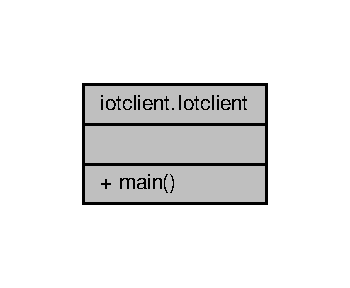
\includegraphics[width=168pt]{classiotclient_1_1Iotclient__coll__graph}
\end{center}
\end{figure}
\subsection*{Static Public Member Functions}
\begin{DoxyCompactItemize}
\item 
static void \hyperlink{classiotclient_1_1Iotclient_a29aeb6bca70f911f937f294096c7b551}{main} (String\mbox{[}$\,$\mbox{]} args)
\end{DoxyCompactItemize}


\subsection{Detailed Description}
\begin{DoxyAuthor}{Author}
ivica 
\end{DoxyAuthor}


\subsection{Member Function Documentation}
\mbox{\Hypertarget{classiotclient_1_1Iotclient_a29aeb6bca70f911f937f294096c7b551}\label{classiotclient_1_1Iotclient_a29aeb6bca70f911f937f294096c7b551}} 
\index{iotclient\+::\+Iotclient@{iotclient\+::\+Iotclient}!main@{main}}
\index{main@{main}!iotclient\+::\+Iotclient@{iotclient\+::\+Iotclient}}
\subsubsection{\texorpdfstring{main()}{main()}}
{\footnotesize\ttfamily static void iotclient.\+Iotclient.\+main (\begin{DoxyParamCaption}\item[{String \mbox{[}$\,$\mbox{]}}]{args }\end{DoxyParamCaption})\hspace{0.3cm}{\ttfamily [inline]}, {\ttfamily [static]}}


\begin{DoxyParams}{Parameters}
{\em args} & the command line arguments \\
\hline
\end{DoxyParams}


The documentation for this class was generated from the following file\+:\begin{DoxyCompactItemize}
\item 
/home/ivica/\+Coding/\+Java/\+C\+S\+\_\+\+I\+O\+T/iotclient/src/iotclient/Iotclient.\+java\end{DoxyCompactItemize}

\hypertarget{classiotserver_1_1Iotserver}{}\section{iotserver.\+Iotserver Class Reference}
\label{classiotserver_1_1Iotserver}\index{iotserver.\+Iotserver@{iotserver.\+Iotserver}}


Collaboration diagram for iotserver.\+Iotserver\+:\nopagebreak
\begin{figure}[H]
\begin{center}
\leavevmode
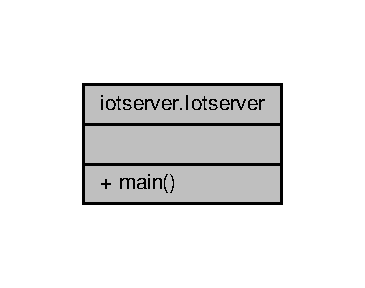
\includegraphics[width=175pt]{classiotserver_1_1Iotserver__coll__graph}
\end{center}
\end{figure}
\subsection*{Static Public Member Functions}
\begin{DoxyCompactItemize}
\item 
\mbox{\Hypertarget{classiotserver_1_1Iotserver_a81c60de8d7f882697a68e4ec04dcd2d8}\label{classiotserver_1_1Iotserver_a81c60de8d7f882697a68e4ec04dcd2d8}} 
static void {\bfseries main} (String\mbox{[}$\,$\mbox{]} args)  throws I\+O\+Exception 
\end{DoxyCompactItemize}


The documentation for this class was generated from the following file\+:\begin{DoxyCompactItemize}
\item 
/home/ivica/\+Coding/\+Java/\+C\+S\+\_\+\+I\+O\+T/iotserver/src/iotserver/Iotserver.\+java\end{DoxyCompactItemize}

\hypertarget{classiotclient_1_1Message}{}\section{iotclient.\+Message Class Reference}
\label{classiotclient_1_1Message}\index{iotclient.\+Message@{iotclient.\+Message}}


Collaboration diagram for iotclient.\+Message\+:\nopagebreak
\begin{figure}[H]
\begin{center}
\leavevmode
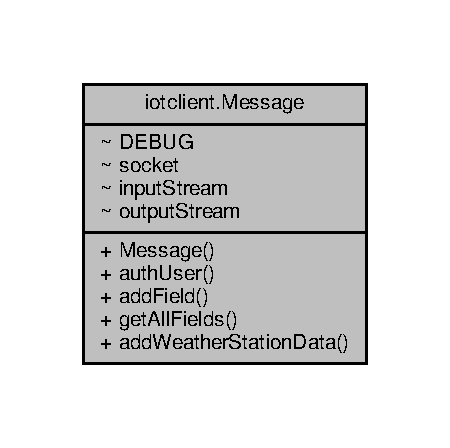
\includegraphics[width=216pt]{classiotclient_1_1Message__coll__graph}
\end{center}
\end{figure}
\subsection*{Public Member Functions}
\begin{DoxyCompactItemize}
\item 
boolean \hyperlink{classiotclient_1_1Message_a4e2ba3e3d5156b8014443aab39e240fc}{auth\+User} (String username, String password)
\item 
J\+S\+O\+N\+Object \hyperlink{classiotclient_1_1Message_aabe363a067aa335d1b00f7587632da52}{add\+Field} (String field\+Name, double longitude, double latitude)
\item 
J\+S\+O\+N\+Array \hyperlink{classiotclient_1_1Message_a22814eaf8f1a8a3bb07b7823c52c83e8}{get\+All\+Fields} ()
\item 
boolean \hyperlink{classiotclient_1_1Message_aab1d4eea6ba3c4172d599aafc5898dfc}{add\+Weather\+Station\+Data} (long weather\+Station\+Id, double temperature, double barometric\+Pressure, double wind\+Speed, double relative\+Humidity, long air\+Quality\+Index)
\end{DoxyCompactItemize}


\subsection{Member Function Documentation}
\mbox{\Hypertarget{classiotclient_1_1Message_aabe363a067aa335d1b00f7587632da52}\label{classiotclient_1_1Message_aabe363a067aa335d1b00f7587632da52}} 
\index{iotclient\+::\+Message@{iotclient\+::\+Message}!add\+Field@{add\+Field}}
\index{add\+Field@{add\+Field}!iotclient\+::\+Message@{iotclient\+::\+Message}}
\subsubsection{\texorpdfstring{add\+Field()}{addField()}}
{\footnotesize\ttfamily J\+S\+O\+N\+Object iotclient.\+Message.\+add\+Field (\begin{DoxyParamCaption}\item[{String}]{field\+Name,  }\item[{double}]{longitude,  }\item[{double}]{latitude }\end{DoxyParamCaption})\hspace{0.3cm}{\ttfamily [inline]}}

Adds a field to a database table.

This method creates J\+S\+O\+N\+Object with key \char`\"{}\+F\+I\+E\+L\+D\+A\+D\+D\char`\"{} having a value of another J\+S\+O\+N\+Object which contains details for a field which are obtained from the parameters of this method. Root object is then sent to a server via send\+With\+Json\+Object\+Return() function which is going to return all details for the newly created field.


\begin{DoxyParams}{Parameters}
{\em field\+Name} & Name of the field as a string \\
\hline
{\em longitude} & Geographical longitude of the field \\
\hline
{\em latitude} & Geographical latitude of the field \\
\hline
\end{DoxyParams}
\begin{DoxyReturn}{Returns}
J\+S\+O\+N\+Object with the details of the newly created field. 
\end{DoxyReturn}
\mbox{\Hypertarget{classiotclient_1_1Message_aab1d4eea6ba3c4172d599aafc5898dfc}\label{classiotclient_1_1Message_aab1d4eea6ba3c4172d599aafc5898dfc}} 
\index{iotclient\+::\+Message@{iotclient\+::\+Message}!add\+Weather\+Station\+Data@{add\+Weather\+Station\+Data}}
\index{add\+Weather\+Station\+Data@{add\+Weather\+Station\+Data}!iotclient\+::\+Message@{iotclient\+::\+Message}}
\subsubsection{\texorpdfstring{add\+Weather\+Station\+Data()}{addWeatherStationData()}}
{\footnotesize\ttfamily boolean iotclient.\+Message.\+add\+Weather\+Station\+Data (\begin{DoxyParamCaption}\item[{long}]{weather\+Station\+Id,  }\item[{double}]{temperature,  }\item[{double}]{barometric\+Pressure,  }\item[{double}]{wind\+Speed,  }\item[{double}]{relative\+Humidity,  }\item[{long}]{air\+Quality\+Index }\end{DoxyParamCaption})\hspace{0.3cm}{\ttfamily [inline]}}

Inputs a weather data to a database table.

This function creates J\+S\+O\+N\+Object with key \char`\"{}\+W\+E\+A\+T\+H\+E\+R\+S\+T\+A\+T\+I\+O\+N\+D\+A\+T\+A\+A\+D\+D\char`\"{} key having a value of another J\+S\+O\+N\+Object containing weather data which is obtained from the parameters of this function.

First parameter, weather\+Station\+Id must be a valid ID number of previously present weather station on the system. Otherwise, adding weather\+Station\+Data would fail and this function will return false.


\begin{DoxyParams}{Parameters}
{\em weather\+Station\+Id} & ID number of weather station this data belongs \\
\hline
{\em temperature} & Temperature \\
\hline
{\em barometric\+Pressure} & Barometric pressure \\
\hline
{\em wind\+Speed} & Wind speed \\
\hline
{\em relative\+Humidity} & Relative humidity, in percentage \\
\hline
{\em air\+Quality\+Index} & Air quality index \\
\hline
\end{DoxyParams}
\begin{DoxyReturn}{Returns}
Boolean value, true if data is successfully entered in a database. 
\end{DoxyReturn}
\mbox{\Hypertarget{classiotclient_1_1Message_a4e2ba3e3d5156b8014443aab39e240fc}\label{classiotclient_1_1Message_a4e2ba3e3d5156b8014443aab39e240fc}} 
\index{iotclient\+::\+Message@{iotclient\+::\+Message}!auth\+User@{auth\+User}}
\index{auth\+User@{auth\+User}!iotclient\+::\+Message@{iotclient\+::\+Message}}
\subsubsection{\texorpdfstring{auth\+User()}{authUser()}}
{\footnotesize\ttfamily boolean iotclient.\+Message.\+auth\+User (\begin{DoxyParamCaption}\item[{String}]{username,  }\item[{String}]{password }\end{DoxyParamCaption})\hspace{0.3cm}{\ttfamily [inline]}}

Authenticates the user based on username and password combination.

This method creates J\+S\+O\+N\+Object with key \char`\"{}\+A\+U\+T\+H\+U\+S\+E\+R\char`\"{} having a value of another J\+S\+O\+N\+Object which contains username and password. Root object is then send to a server via send\+With\+Boolean\+Return() function, which is going to return true if username and password combination is present in a database table.


\begin{DoxyParams}{Parameters}
{\em username} & Username in string format \\
\hline
{\em password} & Password in string format \\
\hline
\end{DoxyParams}
\begin{DoxyReturn}{Returns}
Boolean value, true only if user is successfully authenticated. 
\end{DoxyReturn}
\mbox{\Hypertarget{classiotclient_1_1Message_a22814eaf8f1a8a3bb07b7823c52c83e8}\label{classiotclient_1_1Message_a22814eaf8f1a8a3bb07b7823c52c83e8}} 
\index{iotclient\+::\+Message@{iotclient\+::\+Message}!get\+All\+Fields@{get\+All\+Fields}}
\index{get\+All\+Fields@{get\+All\+Fields}!iotclient\+::\+Message@{iotclient\+::\+Message}}
\subsubsection{\texorpdfstring{get\+All\+Fields()}{getAllFields()}}
{\footnotesize\ttfamily J\+S\+O\+N\+Array iotclient.\+Message.\+get\+All\+Fields (\begin{DoxyParamCaption}{ }\end{DoxyParamCaption})\hspace{0.3cm}{\ttfamily [inline]}}

Gets all fields from a database table.

This function creates J\+S\+O\+N\+Object with key \char`\"{}\+R\+E\+T\+U\+R\+N\+A\+L\+L\+F\+I\+E\+L\+D\+S\char`\"{} having a value of true. Object is then sent to a server via send\+With\+Json\+Array\+Return() function which is going to return J\+S\+O\+N\+Array of J\+S\+O\+N\+Objects, one J\+S\+O\+N\+Object for each field in the database.

\begin{DoxyReturn}{Returns}
J\+S\+O\+N\+Array containing information for all fields in the database table. 
\end{DoxyReturn}


The documentation for this class was generated from the following file\+:\begin{DoxyCompactItemize}
\item 
/home/ivica/\+Coding/\+Java/\+C\+S\+\_\+\+I\+O\+T/iotclient/src/iotclient/Message.\+java\end{DoxyCompactItemize}

%--- End generated contents ---

% Index
\backmatter
\newpage
\phantomsection
\clearemptydoublepage
\addcontentsline{toc}{chapter}{Index}
\printindex

\end{document}
